% Nieuwe uitleg bij de korte Nederlandse hoofdtekst; oudere cijferbijlagen blijven behouden.
\makeatletter
\renewcommand{\fnum@figure}{Figuur \thefigure}
\renewcommand{\fnum@table}{Tabel \thetable}
\makeatother
\ifcsname l@dutch\endcsname\language=\csname l@dutch\endcsname\fi
\section{Vingerkenmerken controleren met de tool}\label{app:feature-tool}
De featuretool vergelijkt gemeten vingerkenmerken met het werkboek voor een gekozen letter. De doelletter bepaalt de vergelijking, niet de modelvoorspelling. Hieronder is ruimte gereserveerd voor een echte foto of screenshot van de tool; dit beeld wordt nog toegevoegd.

\textbf{Buiging:} MCP is de knokkel, PIP het middelste gewricht en DIP het eindgewricht. Een rechte interne hoek nadert $180^\circ$. Vingers zijn gebogen bij hoogstens $130^\circ$ en gestrekt vanaf $150^\circ$; de duim-IP gebruikt $80^\circ$/$155^\circ$. \textbf{Spreiding en kruising} combineren handvlak, diepte en strekking; kruisende 2D-lijnen zijn onvoldoende. \textbf{Duimvorm} gebruikt een eigen palmgerichte regel. \textbf{Contact} gebruikt vingertopafstand gedeeld door pols--middelvingerbasis. Parameters staan in \texttt{config/thresholds.json}; het zijn geen klinisch gevalideerde metingen.

\begin{figure}[h]\centering
\IfFileExists{figures/feature_tool_screenshot.png}{%
  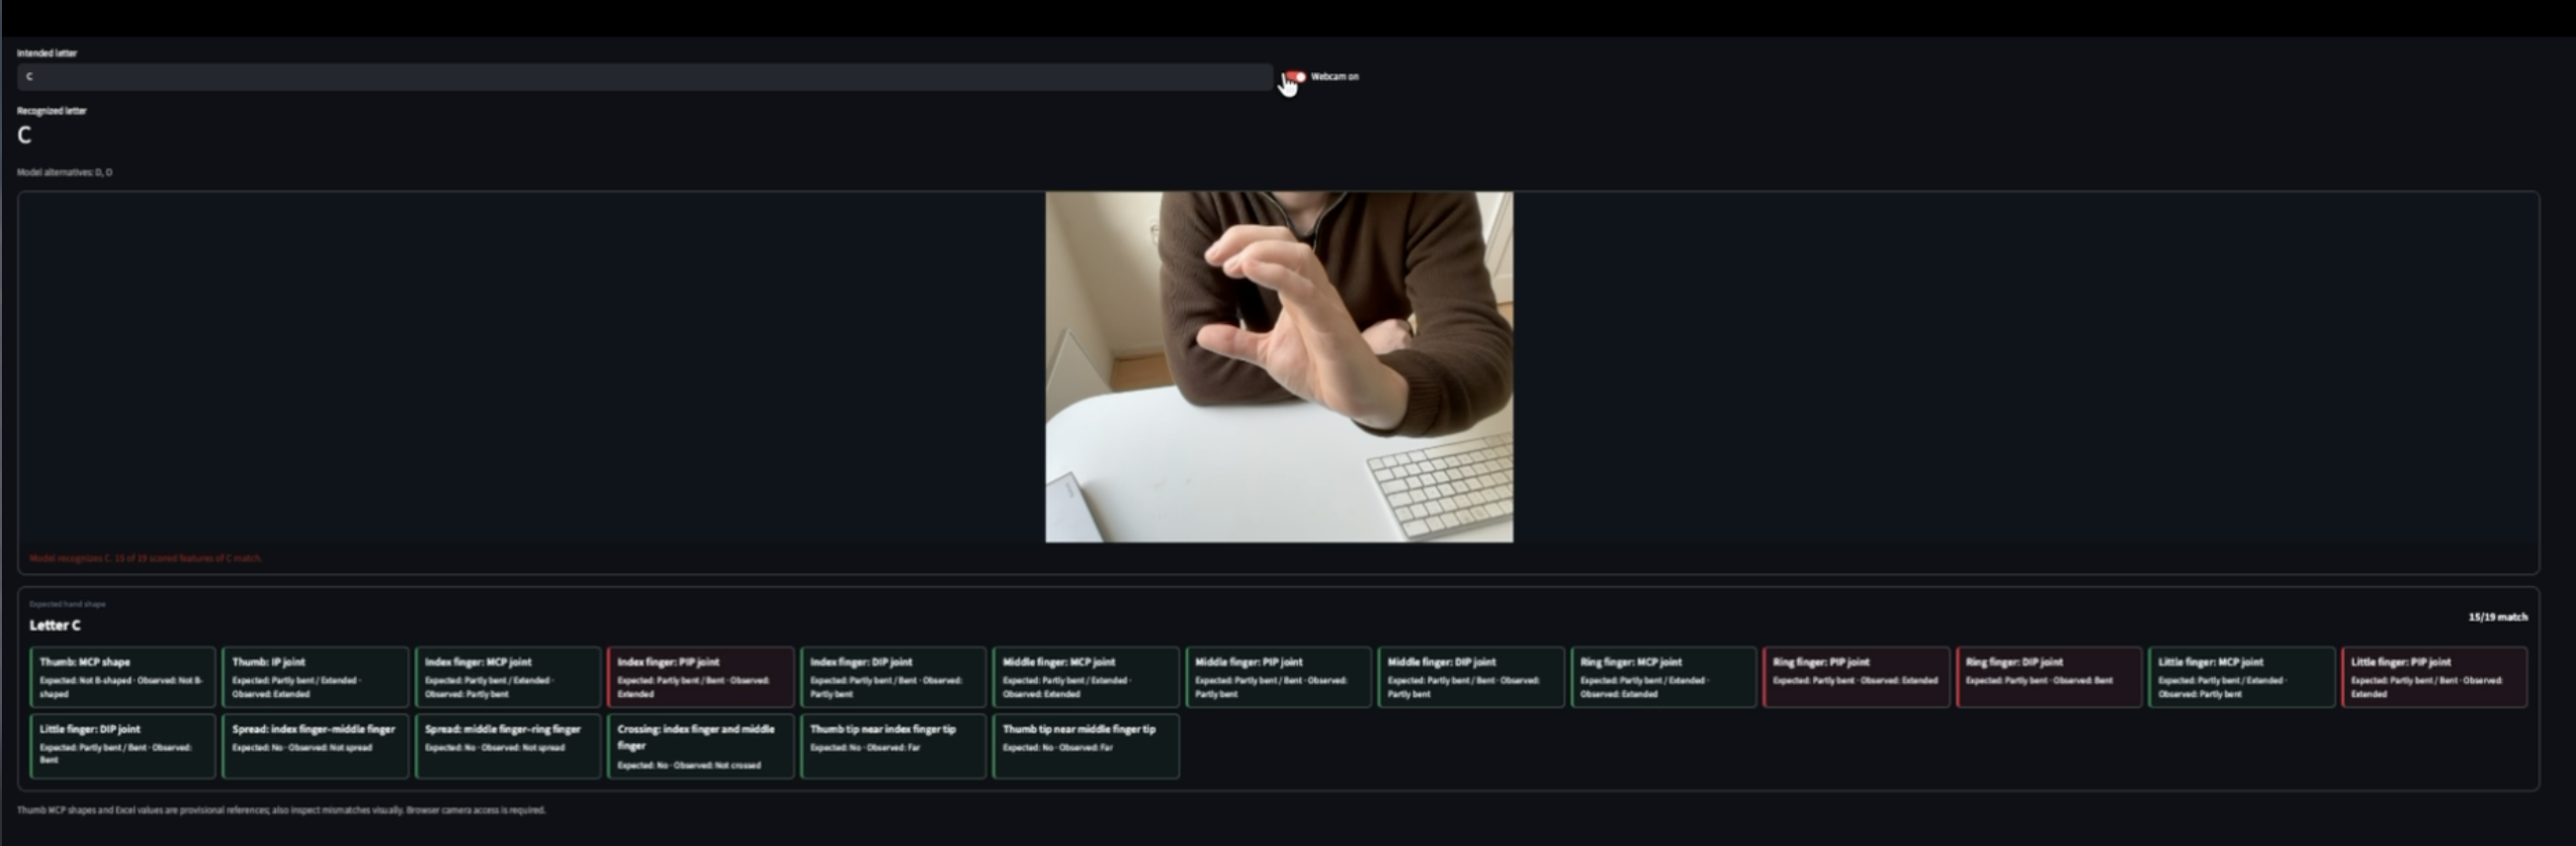
\includegraphics[width=.95\linewidth,height=.55\textheight,keepaspectratio]{figures/feature_tool_screenshot.png}%
}{%
  \fbox{\begin{minipage}[c][5cm][c]{.90\linewidth}\centering
    \textbf{TODO: foto of screenshot van de featuretool}\\[1em]
    Toon het handbeeld met handpunten, de gekozen letter en\\
    de verwachte en gemeten vingerkenmerken.\\[1em]
    Bestand: \texttt{figures/feature\_tool\_screenshot.png}
  \end{minipage}}%
}
\caption{Featurecontrole in de tool. \textbf{TODO:} voeg de eigen opname toe en stem dit bijschrift af op de zichtbare letter en uitkomst. Groen betekent overeenkomst met het werkboek, rood een afwijking. Overeenkomst bewijst niet dat de geschatte handpunten anatomisch correct zijn.}
\label{fig:feature-tool-screenshot}
\end{figure}

\clearpage
\section{Beelden bij de G/H-verwarringen}\label{app:gh-images}
Hieronder staan twee gelabelde datasetvoorbeelden en vier eerder opgeslagen camerabeelden. De bovenste rij illustreert het bronmateriaal; de andere rijen tonen bekende ontwikkelgevallen. Referentie [2] gebruikt wereldgewrichtshoeken. G/H y180 [9] is de afzonderlijke rotatieproef, zonder spiegeltraining, webcamkalibratie of extra voorspelregel. Bij deze twee modellen zijn de getoonde camerabeelden geen trainingsdata. Ze zijn wel eerder bekeken en in andere kalibratieproeven hergebruikt; ze vormen dus geen onafhankelijke test.

\begin{figure}[h]\centering
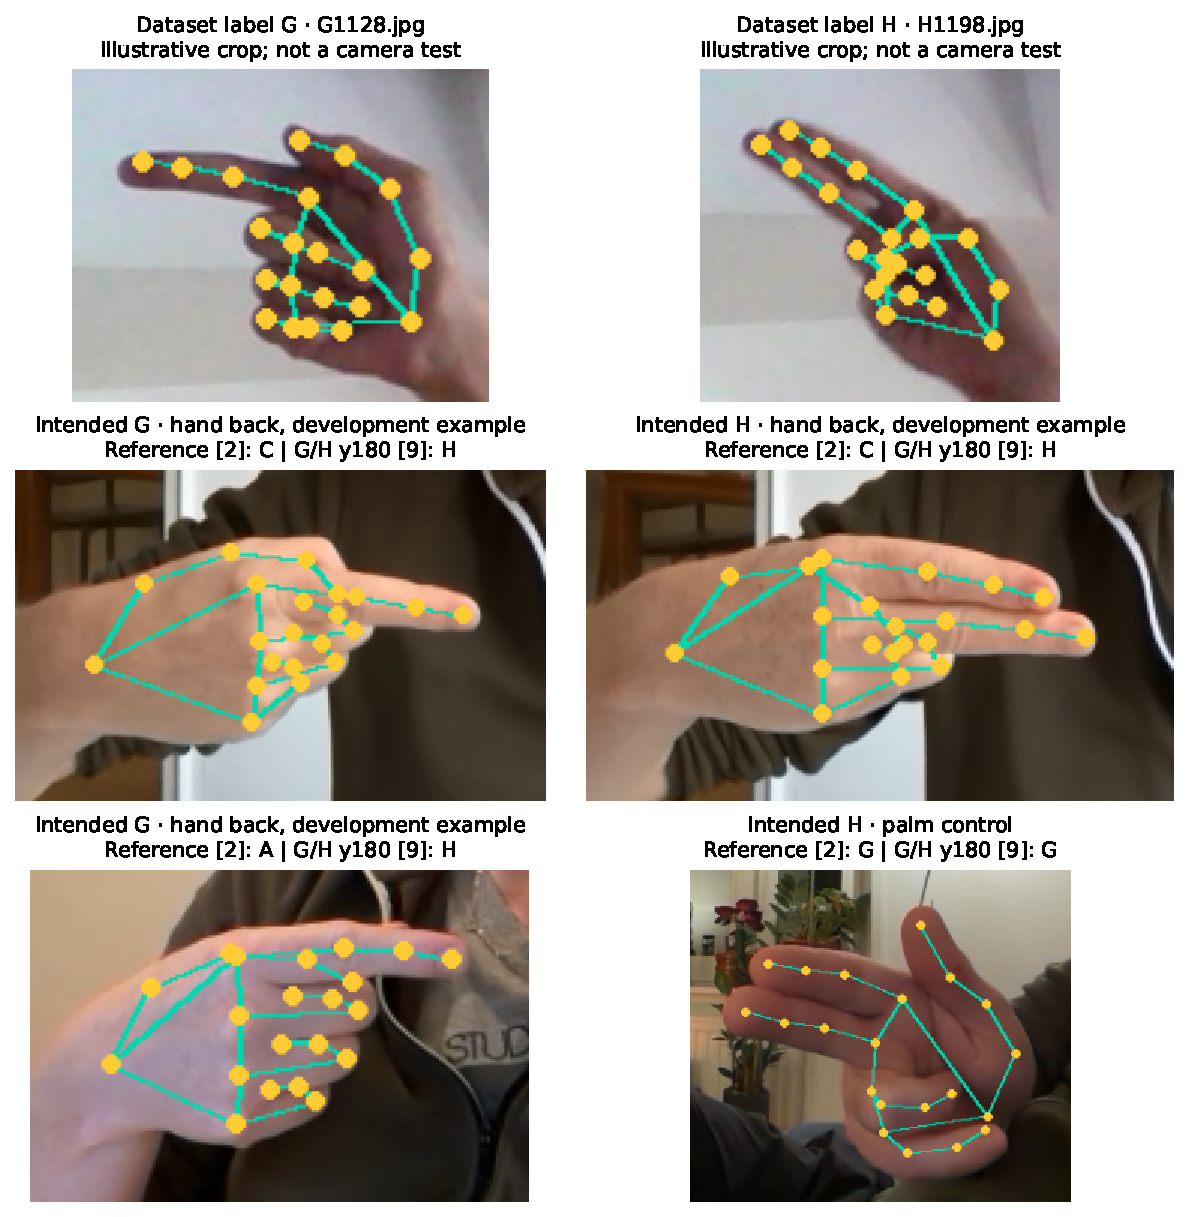
\includegraphics[width=.87\linewidth]{figures/gh_webcam_examples.pdf}
\caption{Handuitsneden met de werkelijk opgeslagen of gecachte handpunten. Datasetlabels zijn overgenomen, niet onafhankelijk op ASL-correctheid beoordeeld. Bij de handrugbeelden herstelt rotatie de bekende H maar blijven beide G-beelden fout. Ook de palmgerichte H wordt G genoemd. De figuur laat verschillen in aanzicht en schattingen zien; zij bewijst niet dat aanzicht de enige oorzaak van de fouten is.}
\end{figure}

\clearpage
\section{Spiegelbeelden en linkshandige presentatie}\label{app:mirror-images}
Er is geen afzonderlijke, gecontroleerde fotoserie van echte linkshandige deelnemers beschikbaar. Wel zijn de oorspronkelijke datasetbeelden en hun horizontale RGB-spiegelingen afzonderlijk gedetecteerd. De onderstaande twee voorbeelden zijn geselecteerd uit de vastgelegde voorspellingen van de spiegelstudie (bijlage L).

\begin{figure}[h]\centering
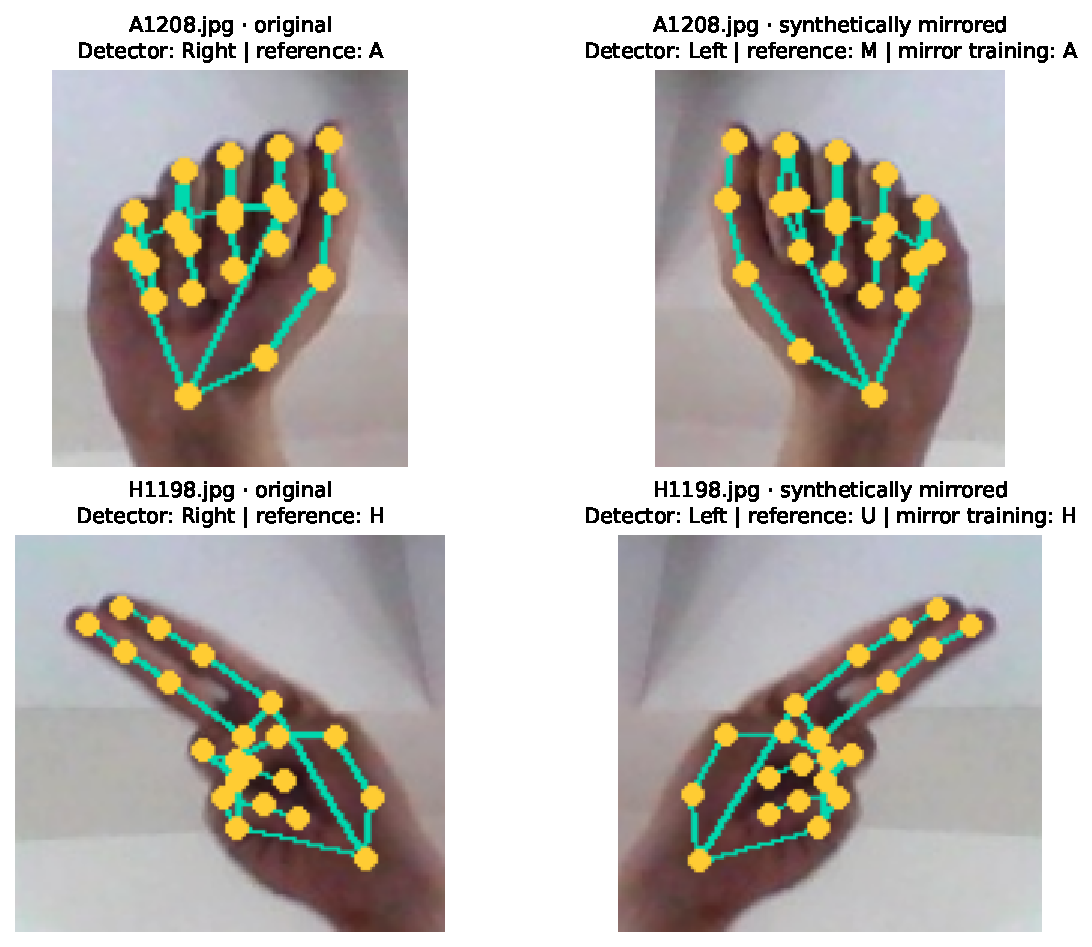
\includegraphics[width=.94\linewidth]{figures/mirror_examples.pdf}
\caption{Links oorspronkelijke A/H-beelden, rechts hun synthetische spiegelingen. De detector geeft respectievelijk Right en Left terug; dit zijn geen door mensen geverifieerde handlabels. Het model zonder spiegeltraining noemt de gespiegelde A een M en H een U; het spiegelgetrainde model herkent beide correct. Dit zijn geselecteerde illustraties, geen nieuwe onafhankelijke deelnemers. Beide bronnen horen bij fold 5; de getoonde voorspellingen komen uit de bijbehorende niet-op-deze-bron-getrainde modellen.}
\end{figure}

Per letter A/H is het eerste passende bron-ID gekozen: geldige Right/Left-detectie, origineel correct, spiegelbeeld fout zonder spiegeltraining en correct daarmee. Deze selectie schat geen succespercentage. Spiegelen maakt een zichtbare handpalm geen handrug. Echte linkshandige gebaren, licht en nieuwe personen blijven afzonderlijke evaluatievragen.

\subsection{Herkomst en herhaling}
\texttt{results/appendix\_visuals\_01/} bewaart bron-ID's, gecontroleerde hashes, uitsneden en featurevergelijkingen. \texttt{appendix\_visuals.py} genereert de figuren; \texttt{--capture} opent de controle in de tool zonder camera of training. De bronbeelden blijven lokaal. De figuren bevatten handuitsneden, geen browser- of accountgegevens.
